\section{Informal overview}

\subsection{Basic types}

\subsubsection{Integer - \lstinline{int}}
    Integers are the basic (and only) numeric type in our language, which serves as the basic building block for higher compositional types.
    \newline \textbf{Examples:} \lstinline{0, 1, 2, 3, 100, 2000, -5, -123}
    
\subsubsection{Boolean - \lstinline{bool}}
    As with many programming languages, Boolean values that can either be true or false and can be used to define decisions and branching in the language.
    \newline \textbf{Examples:} \lstinline{true, false}

\subsubsection{Vector - \lstinline{vec}}
    Vectors in AROS are a composition of two integer components and represent a two-dimensional value, which can be used to define concepts such as size (as values of width and height) or a point on a grid (as coordinates on x and y-axes). 
    \newline \textbf{Examples:} \lstinline{<1,3>, <100,100>, <x,y>}

\subsubsection{List - \lstinline{[]}}
    Lists in AROS are a homogeneous collection of zero to many elements of an arbitrary type. In the context of AROS, they provide a basis for repetition and iteration using higher-order functions. Lists are defined recursively, with two components: a \textit{head} (first element) and a tail (a list containing the rest of the elements).
    \newline \textbf{Examples:}
    \begin{lstlisting}[language=aros,caption=List type examples]
        [int] ints = [1,2,3];
        [vec] vecs = [<1,2>, <3,4>, <5,6>];
    \end{lstlisting}

\subsubsection{Set - \lstinline{\{\}}}
    Similarly to lists, sets are also a collection of homogeneous elements, however, as with mathematical sets, they only allow distinct elements and do not maintain any particular order. Sets are very fundamental in AROS, as they provide the core structure for the definition of grid-based zone layouts. The need for sets as this core structure stems from the nature of defining zone layouts in the form of points on a grid, where non-distinct elements (overlapping points) would bear no meaning.
    \newline \textbf{Examples:} \lstinline|{<1,1>, <1,2>, <1,3>}, {1,2,3}, {true, false}|

\subsubsection{Function - \lstinline{[]}}
    Functions provide an abstraction over expressions, by encapsulating an arbitrary expression inside a local scope. This local scope contains the values of parameters, which are stated when a function is declared and passed into the local scope when the function is called, and the values of local variables declared inside the function body before the return expression. Both the function parameters and the local variables are optional.
    
\newblock
\par 
    In AROS, functions are treated as first-class citizens, and therefore can be used as parameters and/or return expressions of other functions.
    \newline \textbf{Example:}
    \begin{lstlisting}[language=aros,caption=Function type examples]
        (int -> int) addOne = (int) n -> int { n + 1 };
        int two = addOne(1); // two == 2
        
        (-> vec) makeConstVec = () -> vec {
            int x = 10;
            int y = 20;
            <x, y>
        };
        vec myVec = makeConstVec(); // myVec == <10,20>
        
        (int, int -> vec) makeDoublePoint = (int x, int y) -> vec {
           // local declarations 
           int doubled_x = x * 2;
           int doubled_y = y * 2;
           // expression
           <doubled_x, doubled_y>
        }; 
        vec point = makeDoublePoint(2, 2); // point == <4,4>
    \end{lstlisting}

\subsection{Operations}
\subsubsection{Basic arithmetic}
    AROS provides standard binary arithmetic operators for integers: \lstinline{+} for addition, \lstinline{-} for subtraction, \lstinline{*} for multiplication and \lstinline{/} for division. As integers are the only numeric type in AROS, division of two integers is defined as the nearest integer after their division: 
    \begin{equation*}
        \lfloor\frac{a}{b}\rceil
    \end{equation*}
    where $a$, $b$ are integers 
    \newline \textbf{Examples:}
    \begin{lstlisting}[language=aros, caption=Basic arithmetic examples]
        int one = 1;
        int two = one + one;   // two == 2 
        int four = two * two;  // four == 4 
        int four = two * two;  // four == 4 
        int three = 22 / 7;    // three == 3
    \end{lstlisting}
\subsubsection{Comparison operators}
    The comparison operators in AROS are also pretty standard compared to other mainstream programming languages. The equality operator $==$, which can be applied to all types, returns $true$ or $false$ if both operands are structurally equal. Similarly, there is also an inequality operator with symbol $!=$.
    \par The rest of the comparison operators only applied to integers and include:
    \begin{itemize}
        \item Greater than ($>$)
        \item Greater than or equal ($>=$)
        \item Less than ($<$)
        \item Less than or equal ($<=$)
    \end{itemize}
    \textbf{Examples:}
    
    \begin{lstlisting}[language=aros,caption=Comparison operator examples]
        // Integers
        5 == 5                           // true
        5 != 6                           // true
        2 > 1                            // true
        2 >= 1                           // true
        2 >= 2                           // true
        3 < 4                            // true
        3 <= 4                           // true
        3 <= 3                           // true
        
        // Booleans
        true == true                     // true
        true != false                    // true
        
        // Vectors
        <1,3> == <4,5>                   // false
        <1,3> != <4,5>                   // true
        <1,3> == <1,3>                   // true
        
        // Lists
        [1,2,3] == [1,2,3]               // true 
        [3,2,1] == [1,2,3]               // false
        [<1,2>, <3,4>] == [<1,2>, <3,4>] // true
        [<1,2>, <3,4>] == [<3,4>, <1,2>] // false
        
        // Sets
        {1,2,3} == {1,2,3}               // true 
        {3,2,1} == {1,2,3}               // true
        {<1,2>, <3,4>} == {<1,2>, <3,4>} // true
        {<1,2>, <3,4>} == {<3,4>, <1,2>} // true
        
    \end{lstlisting}
\subsubsection{Boolean logic}
    AROS also provides standard binary and unary operators for working with Boolean values, based on predicate logic. These are $and$ (true when both operands true), $or$ (true when either of operands true) and $not$ (negation). The $and$ and $or$ operators are short-circuited, therefore, the evaluation of the second operand may be skipped in case the result can be inferred from just the first operand.  
    \newline \textbf{Examples:}
    \begin{lstlisting}[language=aros,caption=Boolean logic examples]
        5 > 4 and 4 < 5       // true 
        5 > 4 or 5 < 4        // true
        not (5 > 4) and 5 > 4 // false
        not (5 > 4) or 5 > 4  // true
    \end{lstlisting}
\subsubsection{Vector operations}
    The integer arithmetic operators in AROS - $+$, $-$, $*$, $/$ - are overloaded to be also usable on vectors. Applying such operator on two vectors $v1$ and $v2$ will result in a new vector, whose components will be the results of applying the equivalent arithmetic operator pairwise to the respective components of $v1$ and $v2$. 
    \newline Apart from these operations, we can also access the $x$ and $y$ component of a vector by using the $vecx$ and $vecy$ keywords respectively, followed by the vector expression.
    \newline \textbf{Examples:}
    \begin{lstlisting}[language=aros,caption=Vector operation examples]
        vec v1 = <5,3>;
        vec v2 = <2,4>;
        vec added = v1 + v2;       // added == <7,7>
        vec subtracted = v1 - v2;  // subtracted == <3,-1>
        vec multiplied = v1 * v2;  // multiplied == <10,12>
        vec divided = v1 * v2;     // divided == <3,1>
        
        vec vector = <19,20>;
        int x = vecx vector;       // x == 19;
        int y = vecy vector;       // x == 20;
    \end{lstlisting}
\subsubsection{List operations}
    When it comes to (linked) lists in AROS, we can access the $head$ and $tail$ components of a list by using the special keywords `head` and `tail` respectively, followed by an expression of type list. To build a list dynamically, it is possible to use the cons operator ($:$) to prepend a new element onto a list. Additionally, we can also concatenate lists by using the append operator $++$. Given lists $l1$ and $l2$, the concatenation $l1 ++ l2$ evaluates to a new list, which begins with the elements of $l1$, which are followed by the elements of $l2$.
    \newline \textbf{Examples:}
    \begin{lstlisting}[language=aros,caption=List operation examples]
        [int] somePrimes = [13, 17, 19, 23, 29];
        int first = head somePrimes;      // first == 2
        [int] rest = tail somePrimes;       // rest == [3, 5, 7, 11]
        [int] morePrimes =  2 : 3 : 5 : 7 : 11 : []  // demonstrating the cons operator
        [int] myPrimes = morePrimes ++ somePrimes;
        // myPrimes == [2, 3, 5, 7, 11, 13, 17, 19, 23, 29]
    \end{lstlisting}

    
\subsubsection{Set operations}
    As mentioned before, sets are a fundamental feature of AROS and therefore the language natively provides several operators for sets.
    \par The most basic operators are union and intersection with their respective symbols $<>$ and $><$. These follow their mathematical definitions and can be applied to sets with elements of any type.
    \par \textbf{Examples:}
    \begin{lstlisting}[language=aros,caption=Union and intersection examples]
        // Integer sets
        {int} intSet1 = {1,2,3,4,5};
        {int} intSet2 = {4,5,6,7,8};
        {int} intUnion = intSet1 <> intSet2;
        // intUnion == {1,2,3,4,5,6,7,8}
        {int} intInters = intSet1 >< intSet2;
        // intInters == {4,5}
        
        // Vector sets
        {vec} vecSet1 = {<1,2>, <3,4>, <5,6>};
        {vec} vecSet2 = {<3,4>, <5,6>, <7,8>};
        {vec} vecUnion = vecSet1 <> vecSet2;
        // vecUnion == {<1,2>, <3,4>, <5,6>, <7,8>}
        {vec} vecInters = vecSet1 >< vecSet2;
        // vecInters == {<3,4>, <5,6>}
    \end{lstlisting}
    \par Moreover, there are two additional domain specific operators for sets of \textit{vectors}, to facilitate definitions and transformations in the context of points in a grid-based zone layout. Both of these take a set as their first argument, a vector as their second argument, and evaluate to a new set.
    \par The first one is the shift operator with symbol $>>$ which will evaluate to a set of vectors, equivalent to adding the vector argument of $>>$ to each vector in the set argument of $>>$. In the context of the zone, this will \textit{shift} or move the shape defined by the set of vectors.
    \par To give an example, we can show how we can build a shape out of 2 horizontal and 1 vertical lines, using the union and the shift operator: 
    \begin{lstlisting}[language=aros,caption=Examples of the shift operator, label=lst:shift-operator]
        {vec} vertical   = {<0,0>,<1,0>,<2,0>,<3,0>,<4,0>,<5,0>};
        {vec} horizontal = {<0,0>, <0,1>, <0,2>, <0,3>, <0,4>};
        
        // Make new (middle) vertical,
        // by shifting the original 2 coordinates to the right
        {vec} middleVertical = vertical >> (0, 2);
        // middleVertical == {<0,2>,<1,2>,<2,2>,<3,2>,<4,2>,<5,2>}
        
        // Make new (upper) horizontal,
        // by shifting the original 1 coordinate down
        {vec} upperHorizontal = horizontal >> (1, 0);
        // upperHorizontal == {<1,0>, <1,1>, <1,2>, <1,3>, <1,4>};
        
        // Make new (lower) horizontal,
        // by shifting the upper horizontal 3 coordinates down
        {vec} lowerHorizontal = upperHorizontal >> (3, 0);
        // lowerHorizontal == {<4,0>, <4,1>, <4,2>, <4,3>, <4,4>};
        
        // Group the lines into a single shape with union
        {vec} myShape = middleVertical 
                     <> upperHorizontal
                     <> lowerHorizontal;
        // myShape == {
        // <0,2>,<1,0>,<1,1>,<1,2>,<1,3>,<1,4>,<2,2>,
        // <3,2>,<4,0>,<4,1>,<4,2>,<4,3>,<4,4>,<5,2>
        //}
    \end{lstlisting}
    The set of vectors, $myShape$ built in this example, may be seen illustrated in the following figure:
    \begin{figure}[H]
        \centering
        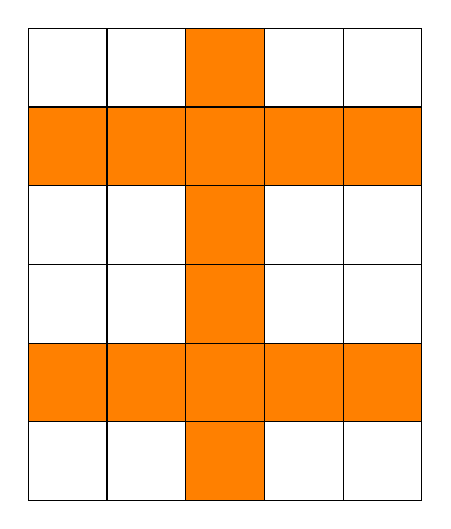
\begin{tikzpicture}[every node/.style={minimum size=1cm-\pgflinewidth, outer sep=0pt}]
            \draw[step=1cm, color=black] (0,0) grid (5,6);
            \node[fill=orange] at (2.5,5.5) {};
            
            \node[fill=orange] at (0.5,4.5) {};
            \node[fill=orange] at (1.5,4.5) {};
            \node[fill=orange] at (2.5,4.5) {};
            \node[fill=orange] at (3.5,4.5) {};
            \node[fill=orange] at (4.5,4.5) {};
            
            \node[fill=orange] at (2.5,3.5) {};
            \node[fill=orange] at (2.5,2.5) {};
            \node[fill=orange] at (2.5,1.5) {};
            \node[fill=orange] at (2.5,0.5) {};
            
            \node[fill=orange] at (0.5,1.5) {};
            \node[fill=orange] at (1.5,1.5) {};
            \node[fill=orange] at (3.5,1.5) {};
            \node[fill=orange] at (4.5,1.5) {};
        \end{tikzpicture}
        \caption{Illustration of shape represented by vector set $myShape$ built in \cref{lst:shift-operator}}
    \end{figure}
    \par The other operator specific to vector-sets is also contextual to defining shapes in the zone, called (and symbolized as) $crop$. The crop operator will remove any vectors from the set (first argument) based on their $x$ and $y$ components, if either of the following is true:
    \begin{itemize}
        \item $v_x > c_x - 1$
        \item $v_y > c_y - 1$
    \end{itemize}
    where $v_x$ , $v_y$ and $c_x$, $c_y$ are $x$ and $y$ components of a vector in the set and the vector argument of the $crop$ operation respectively.
    Effectively, this crops a shape (set of vectors) in a zone into a given width and height, specified in the $x$ and $y$ components of the vector argument of the operation. We can illustrate this on the previously created shape in the following code example:
    
    \begin{lstlisting}[language=aros,caption=Example of using the crop operator, label=lst:cropped-shape]
        {vec} myShapeCropped = myShape crop (5,3);
        // myShapeCropped == {
        // <0,2>,<1,0>,<1,1>,<1,2>,<2,2>,
        // <3,2>,<4,0>,<4,1>,<4,2>
        //}
    \end{lstlisting}
    
Which would result in the following shape:
    
    \begin{figure}[H]
        \centering
        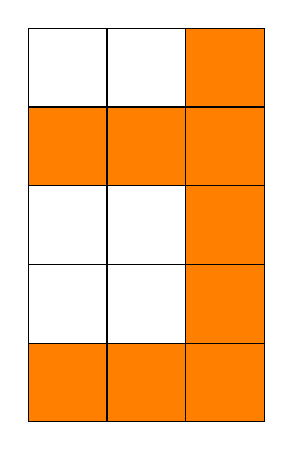
\begin{tikzpicture}[every node/.style={minimum size=1cm-\pgflinewidth, outer sep=0pt}]
            \draw[step=1cm, color=black] (0,0) grid (3,5);
            \node[fill=orange] at (0.5, 0.5) {};
            \node[fill=orange] at (1.5, 0.5) {};
            \node[fill=orange] at (2.5, 0.5) {};
            \node[fill=orange] at (2.5, 1.5) {};
            \node[fill=orange] at (2.5, 2.5) {};
            \node[fill=orange] at (2.5, 3.5) {};
            \node[fill=orange] at (2.5, 4.5) {};
            \node[fill=orange] at (0.5, 3.5) {};
            \node[fill=orange] at (1.5, 3.5) {};
        \end{tikzpicture}
        \caption{Illustration of shape represented by the cropped vector set $myShapeCropped$ built in \cref{lst:cropped-shape}}
    \end{figure}

\subsection{Constructs and Abstractions}
\subsubsection{Functions}
With AROS being a functional language, functions play a fundamental role as abstractions over expressions. Functions can be used to create an expression by constructing it gradually, in several steps (local declaration) in an isolated scope. Functions may be parameterized such that the resulting expression will be constructed and/or evaluated relative to the value(s) provided to the function.

\par{} The main primitive for defining and working with functions is a \textit{lambda} or anonymous function. Lambdas are treated equally to other expressions and act as literals of the function type, in the same way as there are literals for the vector or integer types. Consequently, a function \textit{definition} in AROS, is simply a variable declaration, with a function type and a value in the form of a lambda. An example of this may be seen in the following code listing:
    \begin{lstlisting}[language=aros, float=htb, caption= Function definition by binding a lambda literal to a name]
        (vec, vec -> [vec]) getSquareCoords = (vec bottomLeft, vec topRight) -> [vec] {
            vec topLeft = < (vecx bottomLeft), (vecy topRight) >;
            vec bottomRight = < (vecx topRight), (vecy bottomLeft) >;
            
            [bottomLeft, topLeft, topRight, bottomRight]
        };
    \end{lstlisting}
In the example, a function of type \lstinline{(vec, vec -> [vec])} (two vector parameters + vector list output), named \lstinline{getSquareCoords} has been defined. The function, given two vectors as coordinates of the bottom, left and top right corners of a square returns a list of all the four corners of that square. This example demonstrates how local scope and declarations can be used to define more complicated expression in a much more readable and writable way. 

\par{} Once a function is bound to a name (variable), it is possible to evaluate the function using function application and, for example, bind the evaluated value to a new variable:
    \begin{lstlisting}[language=aros, caption= Function application example]
        [vec] fiveByFive = getSquareCoords(<4,0>, <0,4>);
        // fiveByFive == [<4,0>, <0,0>, <0,4>, <4,4>]
    \end{lstlisting}
\par{} Alternatively, a lambda literal may be evaluated directly, without binding, such as in the following example:
    \begin{lstlisting}[language=aros,float=htb,caption= Direct application of a lambda literal]
        int twoSquared = ((int n) -> int { n * 2 })(2);
        // twoSquared == 4
    \end{lstlisting}

\subsubsection{Conditional expressions}
Decisions based on boolean expressions are facilitated using two main constructs: \lstinline{if} expressions and \lstinline{cond} expressions. As the naming suggests, as the majority of AROS, these are also expressions and therefore may be directly evaluated and bound to variables.

\par As is standard in many programming languages, \lstinline{if} expressions consists of three components: the \textit{condition} and two expressions of same type, call them \lstinline{e1} and \lstinline{e1}. When the entire if expression is evaluated, it will result in either \lstinline{e1} or \lstinline{e2}, based on whether the condition evaluated to \lstinline{true} or \lstinline{false} respectively. An example may be seen in the listing below: 
    \begin{lstlisting}[language=aros, caption= Example of an if expression]
        int x = 10;
        vec a = if (x < 10) { 
            <0,0>    
        } else {
            <10, 10>
        };
        // a == <0,0>
    \end{lstlisting}

\par AROS also makes available another conditional expression, \lstinline{cond}, for situations where the branching consists of more than two branches (and therefore more than one conditions). While this is technically possible to do by nesting \lstinline{if} expressions, \lstinline{cond} provides this functionality in a more concise syntax, giving the users more readability and writability. The following listing contains an example of this construct:

    \begin{lstlisting}[language=aros, caption= Example of a cond expression]
        int x = 100;
        vec a = cond {
            ((x > 0) and (x < 10)) {
                <0,0>
            }
            ((x >= 10)  and (x < 20)) {
                <10,10>
            }
            ((x >= 20) and (x < 30)) {
                <20,20>
            }
            otherwise { <100,100> }
        }; // a == <100, 100>
    \end{lstlisting}
    
\subsubsection{Recursion and Iteration}
In order to execute repetitive computations in a functional style, recursion (function calling itself) can be used. For example, the following code listing includes an implementation of calculating the n-th Fibonacci number recursively:
    \begin{lstlisting}[language=aros, label=lst:fibr, caption= Recursive implementation of calculating n-th Fibonacci number]
        (int -> int) fibr = (int n) -> int {
            cond {
               ((n == 0) or (n == 1)) { n } 
               otherwise { 
                    fibr(n-1) + fibr(n-2)
               }
            }
        }
        int fib5 = fibr(5);
        // fib10 == 55
    \end{lstlisting}

\par{} While \cref{lst:fibr} is sufficient to illustrate recursion, it is a very inefficient implementation. The complexity of this implementation is exponential, due to the repeated recursions stemming from line 5 in \cref{lst:fibr}. The complexity of calculating n-th Fibonacci number can be significantly increased by using an iterative approach. Even though AROS is a functional language and therefore does not support iterative control structures such as a $while$ loop or a $for$ loop, we can make an iterative implementation by passing accumulator values in recursion. The example in 

\newblock

    \begin{lstlisting}[language=aros, label={lst:fibi}, caption= Iterative implementation of calculating n-th Fibonacci number]
        (int, int, int -> int) fibi_h = (int n, int a, int b) -> int {
            cond {
               (n == 0) { a } 
               (n == 1) { b }
               otherwise { 
                    fibi_h(n-1, b, a + b)
               }
            }
        };
        
        (int -> int) fibi = (int n) -> int {
            fibi_h(n, 0, 1)
        };
        
        int fib5 = fibi(5);
        // fib10 == 55
    \end{lstlisting}

\subsubsection{Generic higher-order functions}

\par 
In a functional language paradigm, higher-order function, such as map, filter and fold, are commonly used to solve particular problems. They are in fact, so frequent and versatile, that we have decided to incorporate them into the syntax of AROS. 

\par 
Map takes a function $f$ and a list $l_1$ and applies that function $f$ to every element in the list $l_1$, producing a new list $l_2$. The type scheme of a map is $((\alpha \rightarrow \beta), [\alpha] \rightarrow [\beta])$, meaning that the argument of function $f$ must have the same type as element of list $l_1$ and the return type of function $f$ must be the same as the type of the element of $l_2$. The following example utilizes map to shift every x coordinate of a vector in a list by 1.

\newblock 
\begin{lstlisting}
    (vec -> vec) f = (vec v) -> vec {
        int x = vecx v;
        int y = vecy v;
        <x + 1, y>
    };
    
    [vec] l = [<1,1>, <1,2>, <1,3>];
    
    [vec] new_l = map(f, l); 
    //new_l == [<2,1>, <2,2>, <2,3>]
\end{lstlisting}

\newblock
\par 
Filter takes a predicate (a function $f$, which returns a boolean value) and a list $l_1$ and returns a list $l_2$, consisting of elements of $l_1$ that satisfy the predicate. The type scheme of a filter is $((\alpha \rightarrow Bool), [\alpha] \rightarrow [\alpha])$, meaning that the type of argument of $f$ and the type of elements of both lists $l_1$ and $l_2$ must be equal. The following example utilizes filter to filter out empty sets from a list.

\newblock 
\begin{lstlisting}
    ({vec} -> bool) f = ({vec} s) -> bool {
        s != {}
    };
    
    [{vec}] l = [{<1,1>, <1,2>, <1,3>}, {}, {<0,0>}, {}];
    
    [vec] new_l = filter(f, l); 
    //new_l == [{<1,1>, <1,2>, <1,3>}, {<0,0>}]
\end{lstlisting}

\newblock
\par
A fold (right) takes a function, a starting value (an accumulator) and a list to fold up. The function itself takes two parameters. The function is called with the accumulator and the last element and produces a new accumulator. Then, the function is called again with the new accumulator and the now new last element, and so on. Once we have walked over the whole list, only the accumulator remains, which is what we have reduced the list to. \cite[p. 61]{learn-you-a-haskell-for-great-good} The type scheme of fold right is $((\alpha, \beta \rightarrow \beta), \beta, [\alpha] \rightarrow \beta)$. The following example is an implementation of the above map, using the right fold.

\begin{lstlisting}
    ((vec -> vec), [vec] -> [vec]) map' = ((vec -> vec) f, [vec] l) -> [vec]{
        (vec, [vec] -> [vec]) f' = (vec h, [vec] a) -> [vec] {
            f(h) : a
        }
        foldr(f', [], l)
    }
\end{lstlisting}

\subsubsection{Domain specific constructs}
As mentioned in the previous sections, the key objective of every program written in AROS is to define the map, obstacles and route from the robot's current position to its goal. Therefore, there are two specific constructs that have to be present at the end of every program written in AROS - the grid and route definitions. 

 \par
 The grid definition begins with a $\textit{grid}$ keyword followed by two expressions separated by a comma. The first expression represents the size of the grid and therefore must evaluate to a vector. The second expression must evaluate to a set of vectors because it represents all the obstacles on the grid. Any obstacles defined beyond the size of the grid will simply be discarded. 
 
 \par 
 The route definition begins with a $\textit{route}$ keyword, which is similarly followed by two expressions, separated by a comma. The expressions define the starting and ending position of the path that a robot has to undertake. Both of these expressions have to evaluate to a vector. The following demonstrates the usage of these constructs.
 
 \newblock
 
\begin{lstlisting}
    vec size = <5,5>;
    {vec} obstacles = {<1,1>,<2,2>,<3,3>};
    vec start = <0,0>;
    vec end = <4,4>
    
    grid size, obstacles
    route start, end
\end{lstlisting}